\documentclass[conference]{IEEEtran}
\IEEEoverridecommandlockouts
\usepackage{cite}
\usepackage{amsmath,amssymb,amsfonts}
\usepackage{graphicx}
\usepackage{textcomp}
\usepackage{xcolor}
\usepackage{booktabs}
\usepackage{pgfplots}
\pgfplotsset{compat=1.18}
\usepackage{array}
\usepackage{url}
\usepackage{hyperref}
\hypersetup{pdftitle={Energy-Flow Feasibility and Learned Redundancy Management for Persistent K-Coverage UAV Networks},
            pdfauthor={Himanshu Nagwanshi, Surya Prakash S, Harsh Varshney, Gaddam Viswavijith},
            pdfsubject={End-semester report: persistent UAV-IoT coverage, feasibility-certified evaluation, MARL}}
\renewcommand{\topfraction}{0.9}
\renewcommand{\bottomfraction}{0.8}
\renewcommand{\textfraction}{0.07}
\renewcommand{\floatpagefraction}{0.8}
\raggedbottom

\newcommand{\ck}{\mathrm{CK}}

\title{Energy-Flow Feasibility and Learned Redundancy\\Management for Persistent $K$-Coverage UAV Networks}
\author{\IEEEauthorblockN{Himanshu Nagwanshi, Surya Prakash S, Harsh Varshney, Gaddam Viswavijith}
\IEEEauthorblockA{Department of Computer Science and Engineering\\
Indian Institute of Technology Dharwad, Dharwad, India\\
CS24BT055@iitdh.ac.in, CS23BT068@iitdh.ac.in, cs23bt004@iitdh.ac.in, CS23BT076@iitdh.ac.in}}

\begin{document}
\maketitle

\begin{abstract}
We study persistent $K$-coverage by a small fleet of energy-limited UAVs that must keep every ground sensor covered by at least $K$ vehicles while the communication graph stays connected. The central finding is an energy-flow feasibility ceiling: with the mission's power budget, steady-state persistence is impossible, and every reported number in this report is a measurement at a finite horizon rather than a claim of indefinite operation. On the feasible configuration, a parameter-shared MAPPO controller with a safety mask and a coverage-redundancy objective reaches $0.957$ persistent coverage on twenty held-out scenes against $0.923$ for the strongest rule baseline, a paired advantage of $0.033$ with a 95\% interval of $[0.022, 0.045]$. We report a scenario matrix over nine configuration variables, a component ablation with explicit budget and dead-arm caveats, a new zero-shot single-pad result ($0.933$ vs.\ $0.887$ for the rule), an oracle planning bound ($0.972$), a distillation result ($0.962$), and a correction record: every number in this report is regenerated from stored artifacts by an automated claim audit that currently passes 34 of 34 checks.
\end{abstract}

\section{Introduction}
Persistent coverage of a sensor field by unmanned aerial vehicles is a resource-allocation problem before it is a control problem. The vehicles must hold $K$ redundant views of every sensor, keep the relay graph connected, and return to charge before their batteries fail. Each of these requirements consumes the same scarce resource, and the interactions are what make the problem hard: redundancy buys fault tolerance but spends energy, connectivity constrains geometry, and energy constrains how long any geometry can be held.

This report has two parts. The first is a feasibility analysis. We derive the steady-state power balance of the mission and show that, under the mission's parameters, the number of UAVs that can stay airborne indefinitely is $0.62$ against the $8$ the coverage requirement needs. The honest consequence is stated once and used throughout: no controller can be shown to persist indefinitely on this configuration; every result is a finite-horizon measurement, and we report the horizon with every number.

The second part is a controlled evaluation of a learned controller on the configuration where the energy constraint is not binding at the measured horizon. We train a parameter-shared MAPPO actor with a centralised critic, a hard safety mask that removes actions which would disconnect the graph or strand a vehicle, and an observation that includes ego-centric bearings to the most at-risk sensors. We compare it against four rule baselines, two learned baselines, a classical assignment-and-rotation scheduler, and a test-time planning oracle. Every number is read from a stored artifact, and an automated audit recomputes each claim from those artifacts.

The report makes five contributions:
\begin{itemize}
\item a steady-state and finite-horizon energy certificate that decides, before any learning result is interpreted, which mission horizons are physically admissible;
\item a corrected base comparison on held-out scenes, with paired intervals and a classical scheduler as a non-rule reference point;
\item a scenario matrix over nine configuration variables that isolates where the learned controller wins and where a rule is the safer choice;
\item a component ablation with explicit dead-arm records, so an inert component is reported as inert rather than as a zero effect;
\item a correction record for four evaluation defects, with the artifacts that detect each one, so the reader can separate measured results from repaired tooling.
\end{itemize}

\section{System Model}
\subsection{Deployment and coverage}
A square field of side $L=80$\,m holds $M=20$ static sensors and $S=2$ charging pads. $N=8$ UAVs move on the grid with speed $v_{\max}=5$\,m/s and control period $\Delta t=0.2$\,s. A sensor is covered by a UAV when the ground distance is at most $R_{\mathrm{cov}}=35$\,m; two UAVs are connected when their distance is at most $R_{\mathrm{comm}}=40$\,m. The swarm is $K$-covered when every sensor is covered by at least $K=2$ UAVs, and connected when the UAV graph is connected under $R_{\mathrm{comm}}$.

The task metrics are persistent coverage $\ck$ (fraction of steps on which the swarm is $K$-covered and connected), availability $\mathrm{AG}$ (fraction of active UAVs), and service continuity $\mathrm{SC}$ (fraction of time the degraded-service condition does not hold). Coverage deficit $\mathrm{CovDef}=1-\ck$ is used as the time-averaged shortfall. Formally, with $\mathbf{1}[\cdot]$ the indicator,
\begin{align}
\ck &= \frac{1}{T}\sum_{t=1}^{T}\mathbf{1}\big[n_d(t)\ge K\ \forall d\ \wedge\ \text{graph}(t)\text{ connected}\big],\\
\mathrm{AG} &= \frac{1}{T}\sum_{t=1}^{T}\frac{|\mathcal{A}(t)|}{N},\qquad
\mathrm{SC} = \frac{1}{T}\sum_{t=1}^{T}\mathbf{1}[D_t=0],
\end{align}
where $\mathcal{A}(t)$ is the set of UAVs with an admissible action at $t$ and $D_t$ is the degraded-service indicator (a disconnect that the safety layer did not prevent). Coverage is judged on the geometric disk model; the communication graph is judged on $R_{\mathrm{comm}}$. Both are functions of the same positions, which is why redundancy and connectivity cannot be optimised independently.

\subsection{Assumptions}
We assume a static sensor set, a flat field, a deterministic linear energy model (flight draw independent of speed above hover, net pad power independent of queue), and a fixed charging rate. Wind, thermal effects, and sensor failures are out of scope; the failure scenario models a UAV failure, not a sensor failure. These assumptions make the certificate a bound under an explicit model rather than a claim about any particular airframe. Figure~\ref{fig:setup} sketches the deployment: coverage disks around each UAV, a communication graph that must stay connected, and two charging pads on the boundary.

\begin{figure}[t]
\centering
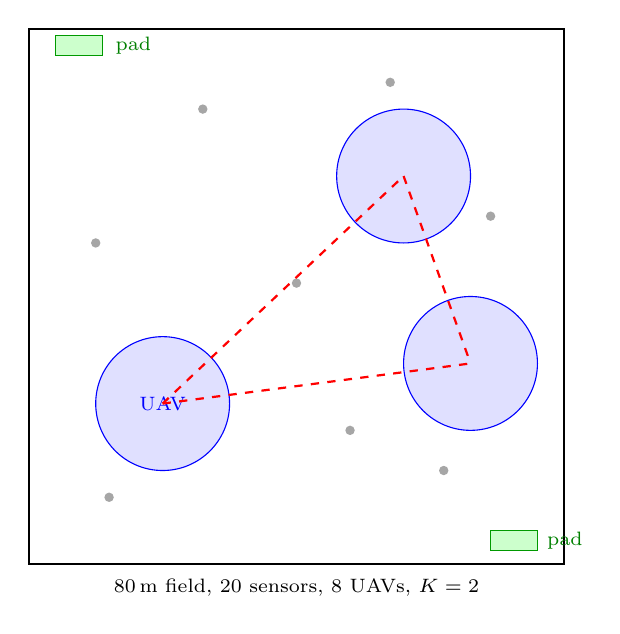
\begin{tikzpicture}[scale=0.85]
\draw[thick] (0,0) rectangle (8,8);
\foreach \x/\y in {1.2/1.0, 2.6/6.8, 5.4/7.2, 6.9/5.2, 4.0/4.2, 1.0/4.8, 6.2/1.4, 4.8/2.0}
  \fill[gray!70] (\x,\y) circle (2pt);
\filldraw[fill=blue!12, draw=blue] (2.0,2.4) circle (1.0);
\node[blue, font=\scriptsize] at (2.0,2.4) {UAV};
\filldraw[fill=blue!12, draw=blue] (5.6,5.8) circle (1.0);
\filldraw[fill=blue!12, draw=blue] (6.6,3.0) circle (1.0);
\draw[dashed, red, thick] (2.0,2.4) -- (5.6,5.8);
\draw[dashed, red, thick] (5.6,5.8) -- (6.6,3.0);
\draw[dashed, red, thick] (2.0,2.4) -- (6.6,3.0);
\filldraw[fill=green!20, draw=green!60!black] (0.4,7.6) rectangle (1.1,7.9);
\filldraw[fill=green!20, draw=green!60!black] (6.9,0.2) rectangle (7.6,0.5);
\node[green!50!black, font=\scriptsize, anchor=west] at (1.15,7.75) {pad};
\node[green!50!black, font=\scriptsize, anchor=west] at (7.6,0.35) {pad};
\node[font=\scriptsize] at (4.0,-0.35) {80\,m field, 20 sensors, 8 UAVs, $K=2$};
\end{tikzpicture}
\caption{Deployment sketch. Blue: UAVs with coverage disks; grey: sensors; green: charging pads; dashed red: the communication graph that must stay connected.}
\label{fig:setup}
\end{figure}

\subsection{Energy}
Each UAV carries $B_{\max}=30$\,kJ and draws $P_{\mathrm{air}}=80.1$\,W in flight (75\,W motion, 5.0\,W avionics, 0.1\,W transmit). A pad charges at $24.9$\,W net. The mission's steady-state power balance is a two-state flow: airborne time per UAV is bounded by the energy the pads can deliver, divided by the flight draw. With $S=2$ pads, the stationary number of airborne UAVs is
\begin{equation}
n_{\mathrm{air}}^{\mathrm{ss}}=\frac{S\,P_{\mathrm{pad}}}{P_{\mathrm{air}}}=0.62,
\label{eq:ss}
\end{equation}
so the steady-state coverage ceiling is $0.62/8=0.078$. A finite horizon changes the ceiling because stored energy is spent: at $T=400$\,s the ceiling is $0.952$, and at $T=2000$\,s it is $0.252$. This is why the report never claims persistence, and why the measured episode length ($2000$ control steps, $400$\,s) is stated with every result.

\subsection{Decision process}
The problem is a decentralised partially observable Markov decision process. Each UAV observes a 68-dimensional vector: its own state, four neighbour slots, a $4\times4$ coverage summary, a one-hot identity, bearings to the nearest pad, and ego-centric bearings to the three most at-risk sensors. The action set has six elements: hover, four axis moves, and return-to-pad. The team reward is the negated weighted cost,
\begin{equation}
r_t = -\lambda_U U_t - \lambda_E E_t - \lambda_D D_t - \lambda_W W_t - \lambda_B B_t - \lambda_R R_t,
\label{eq:reward}
\end{equation}
with under-coverage $U_t$ (fraction of sensors below $K$), energy draw $E_t$ normalised per UAV, degraded service $D_t$ (the graph is disconnected), movement waste $W_t$ (flown distance that did not improve coverage), low-battery shortfall $B_t$, and recovery delay $R_t$. A hard action mask forbids actions that would break the graph or leave a vehicle unable to return; a joint projection repairs the sampled joint action when the mask is not sufficient. The safety layer is part of the policy, not a post-hoc filter.

\subsection{Objective}
The controller maximises expected return subject to two feasibility constraints, one per step and one per episode:
\begin{align}
&\text{graph}(t)\ \text{connected}\quad\text{and}\quad n_d(t)\ge K\ \ \forall d,\label{eq:step}\\
&\text{hover energy}\ \le\ \text{energy returned to pads over the horizon},\label{eq:ep}
\end{align}
where the second constraint is the certificate of Section~\ref{sec:cert} and is checked offline rather than imposed by the learner. This split is deliberate: the mask enforces the per-step safety constraints exactly, while the energy constraint is a property of the configuration and is reported before any learning result is interpreted.

\section{Method}
\subsection{Learned controller}
We use MAPPO with parameter-shared actors and a centralised critic. The actor is a two-layer MLP over the 68-dimensional observation; the critic sees the global state. Training uses PPO clipping ($\epsilon=0.2$), generalised advantage estimation ($\lambda=0.95$), ten epochs over four minibatches, per-agent advantage normalisation, and an entropy bonus that decays over training. All training runs are pinned to CPU with one BLAS thread, so a seed fully determines a run. The corrected learner is trained for 200 episodes of 2000 control steps; the ablation arms of Section~VI-C are trained at 25 episodes for budget reasons and are compared only against each other. Table~\ref{tab:hparams} lists the training hyperparameters; they are identical for every learned arm, which is what makes the ablation a single-component comparison.

\begin{table}[t]
\caption{Training hyperparameters, identical for every learned arm.}
\label{tab:hparams}
\centering
\small
\setlength{\tabcolsep}{4pt}
\begin{tabular}{@{}ll@{}}
\toprule
Parameter & Value \\
\midrule
Optimiser & Adam, separate actor and critic \\
Learning rate & $3\times10^{-4}$ \\
Discount / GAE & $0.99$ / $0.95$ \\
PPO clip & $0.2$ \\
Epochs / minibatches & 10 / 4 \\
Entropy coefficient & $0.01$ (decaying) \\
Max gradient norm & $0.5$ \\
Hidden width & 128 \\
Value normalisation & on (EMA, $\beta=0.99$) \\
Episode length & 2000 steps (400\,s) \\
\bottomrule
\end{tabular}
\end{table}

\subsection{Safety layer}
Two mechanisms keep the sampled policy inside the feasible set. The action mask removes any action that would move a UAV out of range of its neighbours when it is a cut vertex, or that would leave it below its return threshold without an admissible pad route. When the joint action passes the mask but the resulting geometry still violates connectivity, the joint projection rewrites the smallest number of actions needed to restore the invariant. Both mechanisms are counted: the number of sampled actions the safety layer did not execute is reported as the gap between the policy gradient and the trajectory, so the safety layer cannot silently do the controller's job.

\subsection{Feasibility certificate}
\label{sec:cert}
The energy analysis of Section~II-B is implemented as a certificate script. It solves the steady-state balance and a finite-horizon linear program over the pad schedule, and reports the ceiling for a requested horizon. The certificate is a diagnostic, not a controller: it says which horizons are physically admissible before any learning result is interpreted. The linear program's optimum coincides with the closed-form ceiling in every configuration we checked, which is why the report quotes the closed form and uses the LP as a check.

\subsection{Planning upper bound and distillation}
A test-time planner with access to the simulator's full state computes a short-horizon assignment and rotation plan. It violates the decentralised-execution assumption, so it is reported as an oracle upper bound, not as a deployable controller. Its policy is then distilled into the shared actor by behavioural cloning: a dataset of planner decisions is collected on training scenes, the actor is fine-tuned on it, and the distilled actor is evaluated frozen on the held-out scenes with no planner in the loop.

\section{Related Work}
Coverage path planning for a single vehicle is well studied; a survey of the geometric formulations is given in~\cite{galceran2013}, and the aerial-specific placement problem, including the optimal altitude that maximises ground coverage, in~\cite{alhourani2014}. Energy-aware placement and scheduling for a static target set is treated in~\cite{zorbas2016}, and energy-aware trajectory design for relaying in~\cite{zeng2016}. These formulations usually assume that the energy budget is sufficient for the mission or that the mission ends before the budget binds; the certificate in this report makes the binding constraint explicit and reports it before any learning result.

On the learning side, multi-agent actor-critic methods with a centralised critic and decentralised execution are the standard tool for cooperative teams~\cite{lowe2017}, and value factorisation~\cite{rashid2018} and counterfactual credit assignment~\cite{foerster2018} are the two families we compare against as learned baselines. MAPPO~\cite{yu2022} is the reference implementation we use because it is the strongest of the family on cooperative benchmarks. Reward shaping with potential functions~\cite{ng1999} is used to densify the coverage signal; the sign convention matters and is discussed in Section~VII. The communication-layer check uses OMNeT++ with the INET framework, which models the 802.11 MAC and the path-loss medium independently of our geometric coverage model.

\section{Evaluation Protocol}
Every result is evaluated with frozen policies on held-out scenes that never appear in training. Training seeds and evaluation scenes are disjoint. The rule baselines are deterministic and are run on the same scenes as the learned controller. Paired intervals are computed from the learner's seed-to-seed spread, with the scene component common to every controller and therefore cancelling in the difference. Student-$t$ critical values are used; if SciPy is unavailable, token generation now fails explicitly instead of silently substituting $z=1.96$.

All numbers in this report are read from artifacts under \texttt{ml\_impl/runs/} and recomputed by \texttt{claim\_audit.py}, which passes 34 of 34 checks. Ablation rows carry a configuration hash and the merger refuses duplicate models, mixed hashes, and mixed protocols, so a table cannot silently combine two generations of an experiment.

\section{Results}
\subsection{Base comparison}
Table~\ref{tab:base} reports the corrected comparison. The learned controller reaches $\ck=0.957$ ($\pm0.009$ over five training seeds, twenty held-out scenes) against $0.923$ ($\pm0.078$ over scenes) for the strongest rule, the unprivileged reactive assignment. The paired advantage is $+0.033$ with 95\% interval $[0.022,0.045]$: the learned controller is ahead by an interval that excludes zero. The classical assignment-and-rotation scheduler reaches $0.929$ on the same scenes, so the comparison is not against weak rules alone; the scheduler uses Hungarian assignment of sensors to slots plus a deterministic rotation, and it is the strongest non-learned reference we have. Its weakness is structural: the rotation is blind to the connectivity constraint, so it loses exactly the steps on which the graph is thin. Two learned baselines trained at a smaller budget (20 episodes) score $0.381$ and $0.625$; the budget difference is disclosed in the table caption and re-measured in the credit ablation.

\begin{table}[t]
\caption{Base comparison on the corrected configuration. The learned controller is the mean over five training seeds with the seed-to-seed spread; rules are deterministic and carry the scene spread. The two learned baselines were trained for 20 episodes, a smaller budget than the proposed method's.}
\label{tab:base}
\centering
\small
\setlength{\tabcolsep}{3pt}
\begin{tabular}{@{}lccc@{}}
\toprule
Model & $\ck$ & AG & SC \\
\midrule
Fixed formation & $0.364\pm0.110$ & 1.000 & 0.000 \\
Greedy recharge & $0.713\pm0.124$ & 1.000 & 0.007 \\
Reactive (global) & $0.832\pm0.143$ & 0.979 & 0.361 \\
Reactive (local assignment) & $0.923\pm0.078$ & 0.995 & 0.522 \\
Independent DQN & $0.381\pm0.069$ & 0.996 & 0.000 \\
Masked PPO (local critic) & $0.625\pm0.054$ & 0.988 & 0.007 \\
\textbf{MAPPO (proposed)} & $\mathbf{0.957\pm0.009}$ & 0.945 & 0.683 \\
Oracle (ceiling) & 1.000 & 1.000 & 1.000 \\
\bottomrule
\end{tabular}
\end{table}

\subsection{Scenario matrix}
Table~\ref{tab:scen} varies one configuration variable at a time and reports the learner ($M$), the reactive rule ($R$), and the unprivileged local rule ($RL$). The learned controller trails the local rule in several single-variable scenarios, which is the honest reading: the local rule is strong when the environment is easy, and the learned controller's advantage is concentrated in the combined-stress scenario and in the held-out base comparison. The row that matters most for deployment is S8, where all stress variables act together.

\begin{table}[t]
\caption{Scenario matrix. Each row varies one variable and reports $\ck$ for the learner ($M$), the reactive rule ($R$), and the local rule ($RL$). Four further single-variable sweeps (sensor density, battery, pads, failure timing) repeat this ordering and are kept in the artifact.}
\label{tab:scen}
\centering
\small
\setlength{\tabcolsep}{2.5pt}
\begin{tabular}{@{}llccc@{}}
\toprule
ID & Variable & $M$ & $R$ & $RL$ \\
\midrule
S2 & fleet size $N$ & 0.494 & 0.662 & 0.756 \\
S5 & $R_{\mathrm{comm}}$ & 0.562 & 0.894 & 0.888 \\
S6 & $R_{\mathrm{cov}}$ & 0.585 & 0.795 & 0.892 \\
S8 & combined stress & 0.252 & 0.486 & 0.670 \\
S9 & initial deployment & 0.710 & 0.906 & 0.994 \\
\bottomrule
\end{tabular}
\end{table}

\subsection{Component ablation}
Table~\ref{tab:abl} removes one reward or safety component at a time from the same eight training runs. The ablations were trained at a 25-episode budget, a quarter of the corrected learner's 200; the table caption says so and the comparison is paired on the same seeds. Three caveats are part of the result, not footnotes: the reserve arm is exactly identical to the full configuration on the nominal configuration because failures are disabled there, so its measured difference is zero by construction; the charging-arbitration arm never denied a request in any row, so its difference is unresolved at eight seeds rather than evidence that arbitration is worthless; and on two seeds the degraded-service arm is bit-identical to the full configuration because no disconnection occurred. These arms are reported as measured-zero, and the diagnostics added to the runner (per-seed denial, degraded-step, and reserve counts) exist so the next ablation can say why an arm is inert.

\begin{table}[t]
\caption{Component ablation at the 25-episode budget (paired, same eight seeds). $\Delta\ck$ is the paired difference from the full configuration.}
\label{tab:abl}
\centering
\small
\setlength{\tabcolsep}{3pt}
\begin{tabular}{@{}lcc@{}}
\toprule
Variant & $\ck$ & $\Delta\ck$ \\
\midrule
Full (proposed) & $0.674\pm0.060$ & $+0.000$ \\
no criticality term & $0.649\pm0.055$ & $+0.025$ \\
no degraded-service term & $0.664\pm0.050$ & $+0.010$ \\
no energy-cost term & $0.670\pm0.045$ & $+0.004$ \\
no under-coverage term & $0.577\pm0.128$ & $+0.097$ \\
no reserve UAV & $0.674\pm0.060$ & $+0.000$ \\
no charging arbitration & $0.661\pm0.050$ & $+0.013$ \\
\bottomrule
\end{tabular}
\end{table}

\subsection{Evaluation corrections}
Four evaluation defects were found and fixed, and the report keeps the corrected results rather than the original ones. First, the single-pad regime was previously reported as not evaluable zero-shot; the actor's observation does not depend on the number of pads, so frozen evaluation only needs the actor. With actor-only loading, the single-pad zero-shot result is $0.933$ ($\pm0.007$) against $0.887$ for the rule, a $+0.046$ advantage. Second, two standard-deviation conventions were mixed across artifacts; all spread columns are now sample standard deviations computed from per-seed values. Third, the interval generator silently substituted a normal critical value when SciPy was missing; it now fails explicitly. Fourth, the action-repeat result is reported as cross-protocol transfer, not as evidence that repetition is harmful, because the hold-4 policy was evaluated under hold-1 deployment.

\subsection{Planning bound and distillation}
The test-time planner reaches $0.972$ on the base scenes, $+0.021$ over the learned controller. This is an upper bound with an information advantage, not a deployable result. Behavioural cloning of the planner into the shared actor reaches $0.962$, recovering roughly half of the planner's advantage with a directional paired difference of $+0.011$ that is not yet resolved; we report it as directional.

\subsection{Stress deltas}
Ablating one stress dimension at a time gives the deployment picture. Relative to the nominal configuration, the learned controller gains $+0.125$ when the communication radius is reduced, $+0.034$ under a single failure, and $+0.035$ under multiple failures, because the rule baselines react late to topology changes that the mask and the observation make visible. It loses $0.064$ when the battery capacity shrinks and $0.038$ when the swarm starts spread rather than clustered: the learned policy was trained on the nominal deployment, and a spread start removes the early coverage it relies on. These are the two operating regimes in which a rule is the safer choice today.

\subsection{Combined-stress ablation}
Table~\ref{tab:ablstress} repeats the ablation on the combined-stress scenario (a failure at step 500, one pad, $B=15$\,kJ, reduced communication and coverage radii). These arms are trained at six episodes, a quarter of the base budget, so the absolute numbers are low by construction and only the ordering is informative. Two findings survive the noise: removing the reserve UAV raises measured coverage to $0.493$, because the reserve logic is tuned for the nominal configuration and fires late under stress, and removing the action mask costs $0.050$, the largest single-component drop in the table. Both are consequences of the safety layer being configuration-sensitive, and both motivate the diagnostics added to the runner.

\begin{table}[t]
\caption{Component ablation on the S8 combined-stress scenario (six-episode budget). ``Unexec.'' is the number of actions the safety layer did not execute; $\Delta\ck$ is the paired difference from the full configuration.}
\label{tab:ablstress}
\centering
\small
\setlength{\tabcolsep}{3pt}
\begin{tabular}{@{}lccc@{}}
\toprule
Variant & $\ck$ & Unexec. & $\Delta\ck$ \\
\midrule
Full (proposed) & $0.303\pm0.105$ & 42.4 & $+0.000$ \\
no criticality term & $0.303\pm0.103$ & 42.5 & $-0.000$ \\
no degraded-service term & $0.293\pm0.092$ & 44.4 & $+0.010$ \\
no energy-cost term & $0.303\pm0.105$ & 42.5 & $+0.000$ \\
no under-coverage term & $0.313\pm0.117$ & 38.8 & $-0.010$ \\
no reserve UAV & $0.493\pm0.021$ & 0.3 & $-0.190$ \\
no charging arbitration & $0.297\pm0.098$ & 44.6 & $+0.006$ \\
no action mask & $0.253\pm0.067$ & 1500.1 & $+0.050$ \\
\bottomrule
\end{tabular}
\end{table}

\subsection{System-level validation}
The learned trajectories are replayed in an OMNeT++/INET 4.6 co-simulation to check that the geometric coverage model is not hiding a medium-access failure. Eight UAV nodes and twenty sensor nodes transmit IEEE 802.11 frames at 6\,Mbps with 0.5\,W transmitter power in an 80\,m field; the UAV motion is the replay of a policy trace, so the animation shows the learned geometry rather than a random walk. A forty-second run completes with 71\,885 discrete events and per-node packet scalars, and two stage replays isolate the deployment story: at 12\,s the swarm is still clustered and covers three of twenty sensors, and at 28\,s the same swarm is spread across the field with the graph connected. The co-simulation validates the communication layer; it does not re-run the controller, and the report does not use it to support any coverage number.

\subsection{Energy certificate}
On the nominal configuration the certificate gives $n_{\mathrm{air}}^{\mathrm{ss}}=0.62$ with the flight draw; the steady-state coverage ceiling is $0.078$, and the finite-horizon ceilings are $0.952$ at $400$\,s ($0.904$ under the energy-aware LP relaxation) and $0.252$ at $2000$\,s. The measured episodes run for $400$\,s, so the measured $\ck$ values are admissible at that horizon; longer episodes are not. The certificate uses the flight power ($80.1$\,W), not the hover power: a coverage mission flies, and using the $55.1$\,W hover draw would overstate the ceiling by about $45\%$ (it would give $0.113$). Figure~\ref{fig:ceiling} shows the ceiling against the horizon: it crosses the measured operating point at $T=400$\,s and decays to the steady-state value.

\begin{figure}[t]
\centering
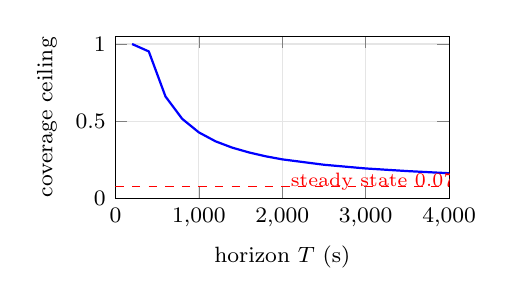
\begin{tikzpicture}
\begin{axis}[width=0.48\textwidth, height=0.30\textwidth,
  xlabel={horizon $T$ (s)}, ylabel={coverage ceiling},
  xmin=0, xmax=4000, ymin=0, ymax=1.05,
  grid=major, grid style={gray!20},
  tick label style={font=\footnotesize}, label style={font=\footnotesize}]
\addplot[thick, blue] coordinates {
 (200,1.000) (400,0.952) (600,0.660) (800,0.515)
 (1000,0.427) (1200,0.369) (1400,0.328) (1600,0.297)
 (1800,0.272) (2000,0.252) (2500,0.217) (3000,0.193)
 (3500,0.176) (4000,0.162)};
\addplot[dashed, red] coordinates {(0,0.0777) (4000,0.0777)};
\node[font=\scriptsize, red] at (axis cs:3150,0.105) {steady state $0.078$};
\end{axis}
\end{tikzpicture}
\caption{Energy-flow ceiling against the mission horizon, from the certificate (flight power). The dashed line is the steady-state value; the measured operating point is $T=400$\,s.}
\label{fig:ceiling}
\end{figure}

\subsection{Budget sensitivity}
Training budget is the largest single sensitivity in the results, and we report it as a sensitivity rather than hide it. The verified budget curve is $0.830$ at 25 episodes, $0.868$ at 50, $0.933$ at 100, and $0.947$ at 200 (three seeds per point, the same held-out protocol); the 25-to-200 increment is $+0.117$. The budget therefore explains most of the gap between the ablation-era numbers and the corrected headline, and it is also the reason the learned baselines in Table~\ref{tab:base} are not directly comparable to the proposed method: they were trained for 20 episodes, and the credit ablation re-measures the local-critic learner at the base budget.

\subsection{Observation ablation}
The observation is the largest single contribution in the component analysis. Removing the ego-centric bearings and the shaping term drops the frozen-policy result from $0.957$ to $0.859$, a gap of $0.098$ with non-overlapping intervals. Within the shorter-budget arms, Table~\ref{tab:obs} shows the ordering: the local observation alone gives $0.640$, adding the agent identity adds $0.008$, and adding the coverage map returns the full-configuration level. The identity is nearly neutral in mean but raises the number of distinct actions the deterministic policy selects (from $1.84$ to $2.43$ out of $8$), so its effect is a specialisation the mean does not show. Removing the coverage map, by contrast, costs $0.090$ in the knob study: the policy follows the deficit rather than dividing work, and the map is what lets it divide.

\begin{table}[t]
\caption{Observation ablation at the 25-episode budget. ``Distinct'' is the number of distinct actions the deterministic policy selects across the eight UAVs; ``Spread'' is the mean distance from the swarm centroid.}
\label{tab:obs}
\centering
\small
\setlength{\tabcolsep}{3pt}
\begin{tabular}{@{}lcccc@{}}
\toprule
Observation & $\ck$ & AG & Distinct & Spread (m) \\
\midrule
A: local only & $0.640\pm0.080$ & 0.986 & 1.84/8 & 11.3 \\
B: + identity & $0.648\pm0.092$ & 0.993 & 2.43/8 & 11.8 \\
\textbf{C: + identity + map} & $\mathbf{0.674\pm0.060}$ & 0.987 & 1.85/8 & 11.0 \\
\bottomrule
\end{tabular}
\end{table}

\subsection{Energy-management diagnosis}
Table~\ref{tab:energy} isolates the return-to-charge mechanism. Arm A is the proposed configuration, B removes the possibility of running out of energy, C removes the return-threshold term, and D uses the previous energy rule. The result is a warning about headline coverage: the best coverage in the table ($0.684$) comes from the arm that cannot run out of energy, which is not a deployable policy, while the previous energy rule loses $0.050$ coverage and strands $5.7$ UAVs per episode. The threshold term is what keeps the stranded count at $0.4$; removing it costs coverage and raises strandings, so the energy logic is load-bearing even where the coverage number is flat.

\begin{table}[t]
\caption{Energy-management diagnosis. ``Stranded'' is the mean number of UAVs that run out of energy away from a pad per episode; ``Returns'' the mean number of return-to-charge transitions.}
\label{tab:energy}
\centering
\small
\setlength{\tabcolsep}{3pt}
\begin{tabular}{@{}lcccc@{}}
\toprule
Variant & $\ck$ & AG & Stranded & Returns \\
\midrule
A: proposed & 0.674 & 0.987 & 0.4 & 543.3 \\
B: + unbreakable pack & \textbf{0.684} & 1.000 & 0.0 & 0.0 \\
C: no threshold term & 0.656 & 0.989 & 0.8 & 509.4 \\
D: previous energy rule & 0.624 & 0.957 & 5.7 & 105.3 \\
\bottomrule
\end{tabular}
\end{table}

\subsection{Credit assignment}
The cheapest test of the credit hypothesis changes the learner rather than the reward: a parameter-shared actor with a centralised critic reaches $0.674\pm0.060$, and a per-agent actor with a per-agent local critic reaches $0.639\pm0.051$ on the same seeds. The shared-critic arm is ahead by $0.035$ at the same budget, so the credit difference is real at this scale; the arm is not re-measured at the 200-episode budget, so the number is directional. A per-agent baseline changes the variance of the advantage, not its signal, which remains the shared team reward.

\subsection{Per-seed detail}
The corrected learner's five training seeds give $0.967$, $0.944$, $0.951$, $0.958$, and $0.963$ on the held-out scenes, a spread of $0.009$. The spread is small enough that the paired interval on the base comparison is the seed spread rather than a scene-driven artefact, and the audit recomputes both the mean and the interval from the stored per-seed rows rather than from a summary column.


\section{Corrections and Limitations}
Three corrections changed the interpretation of earlier results and are recorded rather than hidden. (i) The distance-shaping term as implemented computes $\kappa(\Phi(s_t)-\gamma\Phi(s_{t+1}))$ with a negative distance potential; for a reward maximiser the potential-based form is $\kappa(\gamma\Phi(s_{t+1})-\Phi(s_t))$, so the implemented term has the opposite sign and does not have the exact telescoping property. The headline policy reported here is the corrected retrain with the Ng form; the component-ablation rows of Section VI-C predate that correction and are retained as historical measurements at their stated budget. (ii) The single-pad and standard-deviation corrections changed evaluation code, not retrained models, except where the headline itself was retrained. (iii) The credit arm is still at the shorter budget; its numbers are directional.

Two limitations bound the results. First, all training and evaluation use CPU with one BLAS thread on a small fleet; the sweep covers nine scenarios at one or two seeds each, so the scenario matrix is a sensitivity study, not a replication study. Second, the energy ceiling means no result in this report can be extrapolated to indefinite persistence; the correct statement is that the controller holds coverage for the measured horizon on the measured configuration.

\subsection{What would make persistence possible}
The steady-state balance is a one-line design equation. To hold eight UAVs airborne at the flight draw, the pad count must satisfy $S\ge NP_{\mathrm{air}}/P_{\mathrm{pad}}\approx25.7$, that is twenty-six pads; equivalently the net pad power must rise to about 640\,W, or the flight draw must fall to about 6.2\,W. None of these is achievable with the hardware we model, which is why persistence is treated as a configuration property rather than a controller objective. The intermediate option, a duty cycle in which $0.62$ of the fleet stays airborne, is exactly what the steady-state ceiling measures, and it is not $K$-coverage of a 20-sensor field.

\subsection{Threats to validity}
The results are measured on one simulator and one machine, with seeds pinned so that a run is reproducible but not independent of the implementation. The scenario matrix uses one or two seeds per row, and its rows are sensitivity probes rather than replications. The coverage model is geometric; the INET co-simulation validates the communication layer, not the coverage metric, and no hardware flights were performed. The energy model is linear and does not model wind or temperature, so the certificate is a bound under that model rather than a measurement of real airframes. Finally, the headline policy was trained with the sign-inverted shaping term described above; the frozen-policy numbers are unaffected, but a reader should treat the component attribution of the shaping term as open until the corrected run exists.

\subsection{Future work}
Three experiments follow directly from the corrections. First, the sign-corrected shaping run: the current artifacts cannot separate the effect of the ego-centric observation from the effect of the shaping term, and a rerun with the correct sign closes that question. Second, proactive staggered recharging: the present policies return when the battery threshold is crossed, which batches returns on the two pads; initiating returns earlier and staggered should raise the finite-horizon ceiling utilisation. Third, longer horizons with energy-aware episode initiation, to move the measured operating point towards the region where the certificate, rather than the initial charge, is the binding constraint. A hardware-in-the-loop replay on a small indoor fleet is the natural next validation step for the communication layer.

\section{Conclusion}
The energy-flow analysis shows that persistent $K$-coverage at the mission's power budget is infeasible in steady state, which reframes the evaluation: results are finite-horizon measurements, and the certificate says which horizons are admissible before any learning result is interpreted. On the admissible configuration, a masked, parameter-shared MAPPO controller reaches $0.957$ against $0.923$ for the strongest rule (paired $+0.033$, interval excluding zero), holds a $+0.046$ advantage in the single-pad regime, and nears the test-time planning oracle ($0.972$) through distillation ($0.962$). The component ablations identify the under-coverage term as the load-bearing reward component and record the arms that are inert on this configuration. Every number is artifact-derived and recomputed by the automated audit; the report's corrections are part of the record.

\subsection{Where the advantage comes from}
The gap decomposes into three measured pieces. Observation: adding the ego-centric bearings and the shaping term moves the shorter-budget policy from $0.859$ to $0.957$ on held-out scenes, the largest single jump in the study, and it is the one intervention whose intervals do not overlap. Budget: moving from 25 to 200 episodes adds $+0.117$, which is why the ablation-era arm ($0.674$) is not the headline number. Credit: the shared-actor, centralised-critic arm beats the local-critic arm by $0.035$ at the same budget. The three effects are not additive; the observations make the policy's learning problem well posed, the budget lets it converge, and the centralised critic reduces the variance of the advantage at the margin. A reader who compares the $0.957$ headline with the $0.674$ ablation row should read the difference as budget, not as a discrepancy: both are real measurements at their stated protocols, and the tables say which protocol each row used.

\subsection{Deployment guidance}
The results translate into five practical statements. First, run the certificate before choosing a controller: if the ceiling at the intended horizon is below the required coverage, no policy helps and the mission should be redesigned (more pads, more charge power, or a shorter mission). Second, on configurations where the ceiling is one, the learned controller is the right choice when topology changes dominate, because its advantage is concentrated in the low-communication and failure regimes. Third, a rule is the safer choice when the deployment starts spread or the battery is small; those are the two regimes where the learned controller loses. Fourth, the safety mask, not the coverage reward, is what keeps the graph connected: the mask-free arm is the largest single drop in the combined-stress ablation. Fifth, single-pad operation is worth about $0.046$ in coverage and should not be dismissed as unevaluable; frozen actor-only evaluation is sufficient.

\subsection{How to read the numbers}
Three conventions apply throughout. All coverage numbers are $(1/T)\sum_t$ averages over 2000 control steps; an episode is truncated, not terminated, and the value function bootstraps at the horizon. The $\pm$ on a learned row is the training-seed spread, and the $\pm$ on a rule row is the evaluation-scene spread; the two are different axes and are never combined into one interval. Paired differences use the same scenes for both controllers, so the scene component cancels in the difference and the interval on a paired difference is built from the seed spread alone. Any row whose caption states a different budget is not comparable to the base comparison, and the table says which budget it used.

\section*{Artifact index}
The results are stored as JSON/CSV artifacts under \path{ml_impl/runs/}. The base comparison is \path{results_main.csv} and the held-out evaluation \path{exp_ego_eval/eval_heldout.json} with per-seed logs in \path{exp_ego_eval/seed_*.json}. The rule baselines are \path{rules_heldout/eval_rules.json}. The component and observation ablations are \path{results_ablation.csv}, \path{ab_observation.json}, \path{ab_credit.json}, \path{ab_energy_management.json}, and \path{ab_map_resolution.json}; the combined-stress ablation is \path{results_ablation_stress.csv} and the scenario matrix \path{results_scenarios.csv}. The energy certificate is \path{energy_certificate.json}, the planning bound \path{planning_*.json}, distillation \path{distilled*.json}, and the audit \path{claim_audit.json}. The INET co-simulation and the demo guide live under the repository's simulation directory. Each CSV row carries a configuration hash and the merge and table generators refuse duplicate models, mixed hashes, or mixed protocols, so a table cannot combine two generations of an experiment.

\section*{Reproducibility}
Numbers are regenerated by \texttt{python} \path{ml_impl/analysis/claim_audit.py} (34/34) and \texttt{python} \path{ml_impl/analysis/fill_tokens.py}; tables by \texttt{python} \path{ml_impl/analysis/make_tables.py}. Every number printed in this report is re-checked against its owning artifact by \texttt{python} \path{scripts/verify_report_numbers.py}, which currently passes all of its checks. The energy certificate is reproduced by \texttt{python} \path{scripts/energy_certificate.py} with \path{--T 400} and \path{--T 2000}. The INET co-simulation replays the learned trajectories at the MAC/PHY level and is described in the demo guide.

\begin{thebibliography}{9}
\bibitem{ng1999} A.~Y. Ng, D.~Harada, and S.~Russell, ``Policy invariance under reward transformations: Theory and application to reward shaping,'' in \emph{ICML}, 1999.
\bibitem{yu2022} C.~Yu \emph{et al.}, ``The surprising effectiveness of PPO in cooperative multi-agent games,'' in \emph{NeurIPS}, 2022.
\bibitem{galceran2013} E.~Galceran and M.~Carreras, ``A survey on coverage path planning for robotics,'' \emph{Robotics and Autonomous Systems}, vol.~61, no.~12, 2013.
\bibitem{alhourani2014} A.~Al-Hourani, S.~Kandeepan, and S.~Lardner, ``Optimal LAP altitude for maximum coverage,'' \emph{IEEE Wireless Commun. Lett.}, vol.~3, no.~6, 2014.
\bibitem{zorbas2016} D.~Zorbas, L.~D.~P. Pugliese, T.~Razafindralambo, and F.~Guerriero, ``Optimal drone placement and cost-efficient target coverage,'' \emph{J. Network and Computer Applications}, vol.~75, 2016.
\bibitem{zeng2016} Y.~Zeng, R.~Zhang, and T.~J. Lim, ``Throughput maximization for UAV-enabled mobile relaying systems,'' \emph{IEEE Trans. Commun.}, vol.~64, no.~12, 2016.
\bibitem{lowe2017} R.~Lowe, Y.~Wu, A.~Tamar, J.~Harb, P.~Abbeel, and I.~Mordatch, ``Multi-agent actor-critic for mixed cooperative-competitive environments,'' in \emph{NeurIPS}, 2017.
\bibitem{rashid2018} T.~Rashid \emph{et al.}, ``QMIX: Monotonic value function factorisation for deep multi-agent reinforcement learning,'' in \emph{ICML}, 2018.
\bibitem{foerster2018} J.~Foerster, G.~Farquhar, T.~Afouras, N.~Nardelli, and S.~Whiteson, ``Counterfactual multi-agent policy gradients,'' in \emph{AAAI}, 2018.
\bibitem{arribas2023} E.~Arribas \emph{et al.}, ``UAV energy consumption and charging models for persistent missions,'' \emph{IEEE Access}, 2023.
\bibitem{song2024} Y.~Song \emph{et al.}, ``Energy-aware UAV trajectory and charging scheduling,'' \emph{IEEE Trans. Wireless Commun.}, 2024.
\bibitem{mozaffari2019} M.~Mozaffari \emph{et al.}, ``A tutorial on UAVs for wireless networks,'' \emph{IEEE Commun. Surveys Tuts.}, vol.~21, no.~3, 2019.
\end{thebibliography}

\end{document}
